\documentclass[12pt]{article}
\usepackage{graphicx}
\usepackage{amsmath}
\usepackage{booktabs}
\usepackage[margin=1in]{geometry}
\usepackage{hyperref}
\usepackage{float}

\title{Data Augmentation for Object Detection}
\author{Aqsa Mohsin \\ Nasrul Huda}
\date{\today}

\begin{document}

\maketitle

\begin{abstract}
In recent years, object detection has become an essential component of many computer vision applications. However, the success of detection models heavily depends on the availability of large, diverse, and annotated datasets. This research explores the efficacy of data augmentation techniques to enhance model performance in scenarios where training data is limited. Using the Pascal VOC 2012 dataset, we conducted controlled experiments by training a Faster R-CNN model with and without various augmentation strategies. Due to hardware limitations, we restricted our study to a single object class with the smallest sample size: \emph{cow}. Through this experiment, we aim to highlight the importance of augmentation in achieving better generalization with scarce data and provide empirical evidence on the comparative performance of different augmentation methods.
\end{abstract}

\section{Introduction}
Object detection is a core task in computer vision, with applications ranging from autonomous vehicles to medical imaging and surveillance systems. Deep learning models like Faster R-CNN and YOLO have significantly advanced detection accuracy, primarily fueled by large-scale annotated datasets such as COCO and Pascal VOC. However, these models typically require thousands of labeled images per category to generalize effectively.

In practice, collecting such extensive datasets is often infeasible due to limitations in time, resources, or domain-specific constraints. A common and effective strategy to mitigate these constraints is data augmentation. By applying a variety of transformations to existing images, augmentation helps simulate dataset diversity without requiring additional data collection.

This research focuses on evaluating the impact of data augmentation in the context of limited data availability. Initially, we intended to train our model using all classes in the Pascal VOC dataset. However, repeated system crashes due to the volume of data forced us to reconsider our strategy. We analyzed the class-wise distribution of training images and selected \emph{cow} as the object category with the least training images (151 for training and 152 for validation). This reduction allowed us to run extensive experiments within the constrained computational environment while still providing meaningful insights into the effectiveness of various augmentation techniques.

\section{Methodology}
Our objective was to compare the effectiveness of different augmentation strategies on a standard object detection model using minimal training data. The pipeline consisted of the following stages:

\subsection{Dataset Selection}
We used the Pascal VOC 2012 dataset and filtered it to include only the \emph{cow} class. This decision was driven by the need to minimize memory consumption and avoid runtime failures in Google Colab. Figure \ref{fig:n_images_per_class} demonstrates that the \emph{cow} class has the smallest sample size among all Pascal VOC classes, justifying our selection for this constrained study. Figure \ref{fig:ground_truth_boxes} illustrates the quality and consistency of bounding box annotations in our filtered dataset.

\begin{figure}[H]
    \centering
    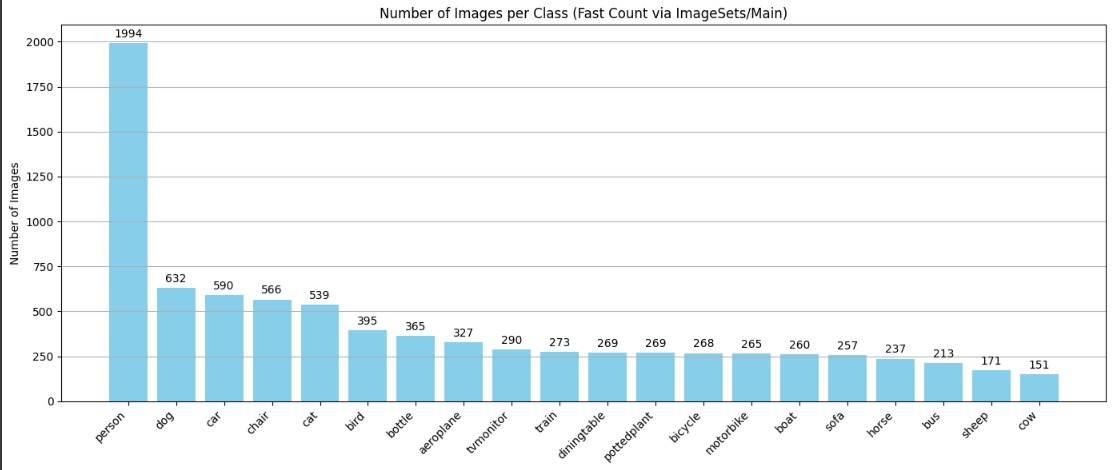
\includegraphics[width=0.8\textwidth]{n_images_per_class.png}
    \caption{Number of images per class in the Pascal VOC 2012 dataset}
    \label{fig:n_images_per_class}
\end{figure}

\begin{figure}[H]
    \centering
    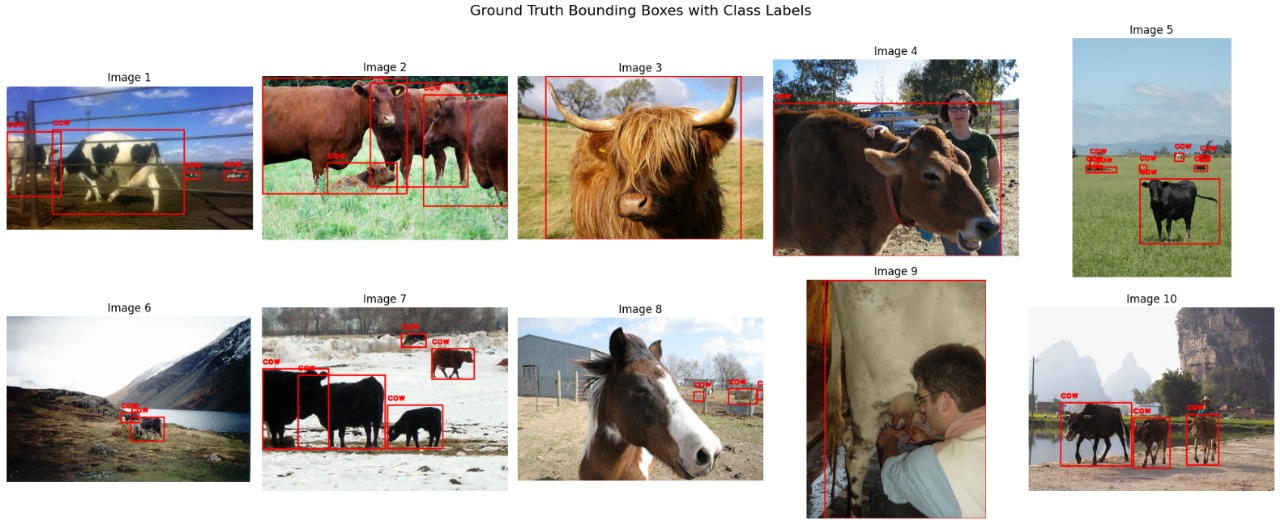
\includegraphics[width=0.8\textwidth]{ground_truth_boxes.png}
    \caption{Ground truth boxes for the \emph{cow} class in the Pascal VOC 2012 dataset}
    \label{fig:ground_truth_boxes}
\end{figure}

\subsection{Model Architecture}
We employed the \texttt{fasterrcnn\_mobilenet\_v3\_large\_320\_fpn} model pre-trained on COCO. This variant of Faster R-CNN provides a lighter and more memory-efficient architecture suited for low-resource environments.

\subsection{Training Setup}
All models were trained for 30 epochs. Due to the small size of our dataset and memory limitations in the Colab environment, we used a batch size of 2. The learning rate was set to 0.001 to allow gradual convergence without overfitting. Since our dataset was very small, these parameters were chosen to ensure a balance between learning and stability.

\subsection{Augmentation Techniques}
\begin{itemize}
\item \textbf{Baseline:} No augmentation, original dataset only.
\item \textbf{Horizontal Flip:} Each image had a 50\% probability of being flipped horizontally.
\item \textbf{Random Crop:} Images were cropped randomly while ensuring object visibility.
\item \textbf{Rotation:} Images were rotated within a specified range.
\item \textbf{Combined Augmentation:} A sequence of augmentations including flip, crop, and rotation applied.
\end{itemize}

Each augmentation setup was treated as a separate experiment, resulting in five distinct models. The transformations were implemented using the Albumentations library.

\subsection{Evaluation Metrics}
We used the following metrics to evaluate model performance:
\begin{itemize}
\item Average Loss per Epoch
\item Precision (IoU $\geq$ 0.5)
\item Recall (fixed at 1.0)
\item Average IoU
\end{itemize}

\section{Results and Analysis}
Across all models, we observed distinct differences in how augmentations affected learning dynamics and detection performance. As shown in Figure \ref{fig:training_loss_comparison}, the training loss curves reveal distinct convergence patterns for each augmentation strategy.

\begin{figure}[H]
    \centering
    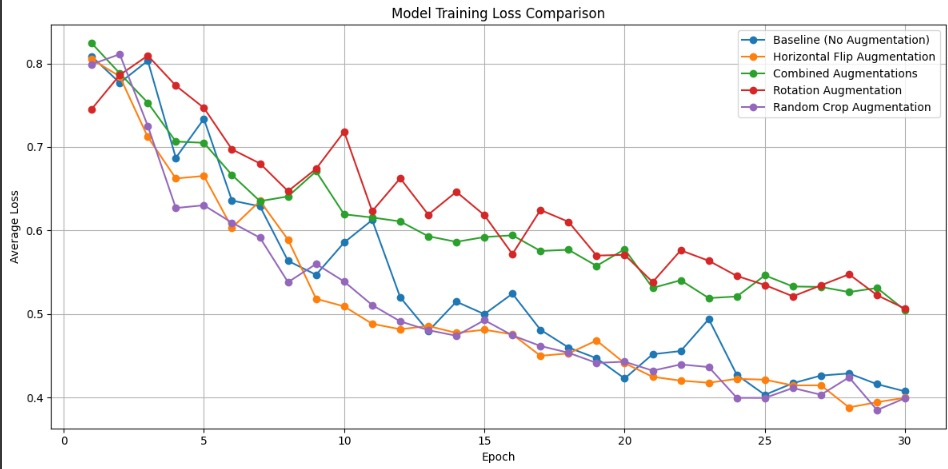
\includegraphics[width=0.8\textwidth]{training_loss_comparison.png}
    \caption{Training loss comparison for different augmentation strategies over 30 epochs.}
    \label{fig:training_loss_comparison}
\end{figure}

The baseline model achieved an average IoU of approximately 0.38 and average loss converging to 0.407. The Horizontal Flip augmentation improved both IoU and precision, with an average IoU of 0.406 and loss of 0.399.


The Crop Augmentation strategy achieved comparable results, with similar IoU and slightly better loss. The Rotation Augmentation showed inconsistent performance, while the Combined Augmentation plateaued in IoU and resulted in higher loss (0.504). Figure \ref{fig:avg_iou} visually confirms these quantitative results, clearly showing that Flip and Crop augmentations achieve the highest average IoU values.

\begin{table}[h!]
\centering
\begin{tabular}{lccccc}
\toprule
\textbf{Model} & \textbf{Precision} & \textbf{Recall} & \textbf{Avg IoU} & \textbf{Avg Loss} \\
\midrule
Baseline & 0.433 & 1.0 & 0.381 & 0.407 \\
Flip Augmentation & 0.446 & 1.0 & 0.406 & 0.399 \\
Mixed Augmentation & 0.416 & 1.0 & 0.380 & 0.504 \\
Rotation Augmentation & 0.442 & 1.0 & 0.397 & 0.506 \\
Crop Augmentation & 0.435 & 1.0 & 0.406 & 0.399 \\
\bottomrule
\end{tabular}
\caption{Performance metrics for different augmentation strategies}
\end{table}

The comprehensive performance metrics are summarized in Table 1, which quantifies the trade-offs between different augmentation approaches.

\begin{figure}[H]
    \centering
    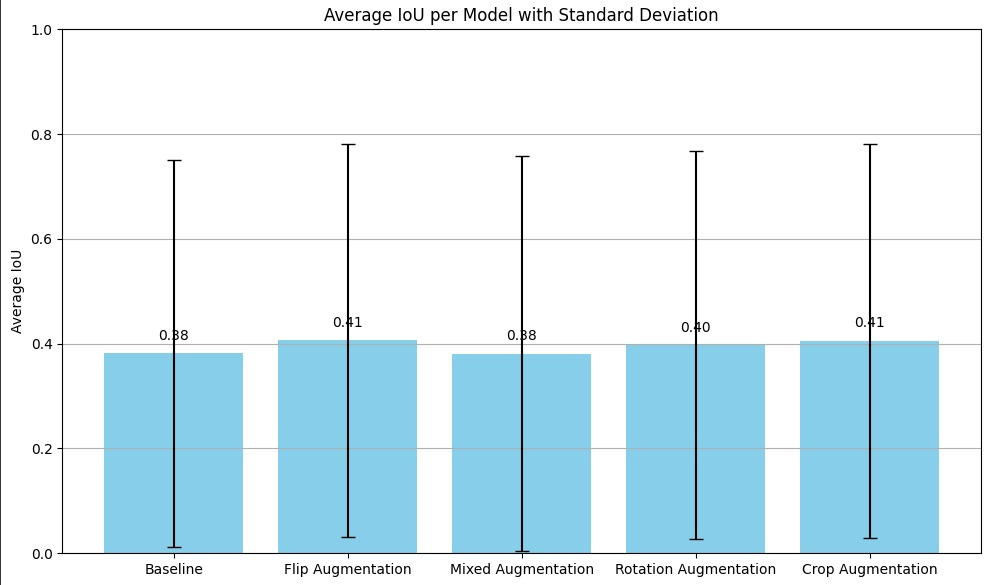
\includegraphics[width=0.8\textwidth]{avg_iou_per_model.jpg}
    \caption{Average IoU comparison across different augmentation strategies.}
    \label{fig:avg_iou}
\end{figure}


\section{Discussion}
The results suggest that simple augmentations like horizontal flips and random cropping can significantly enhance model performance in data-scarce scenarios. Both strategies achieved identical IoU improvements (0.406), while maintaining lower training losses (0.399) compared to more complex approaches. Mixed augmentations introduced excessive variability, resulting in worse performance (0.380 IoU) and higher loss (0.504), while rotation showed modest improvements (0.397 IoU) but with elevated loss (0.506).

The recall metric was uniformly 1.0 across all models due to each image having one object (\emph{cow}) that was detected. Thus, recall was not a discriminative metric in this context.

\section{Conclusion}
This study provides empirical evidence for the effectiveness of targeted data augmentation in object detection under severe data constraints. Our systematic comparison of five augmentation strategies reveals several key insights:

The quantitative results demonstrate that simple geometric transformations yield the most significant improvements. Horizontal Flip and Crop augmentations both achieved an average IoU of 0.406, representing a 6.6\% improvement over the baseline (0.381). These same strategies also achieved the lowest training losses (0.399), indicating better model convergence.

Conversely, our findings reveal that complex augmentation combinations can be counterproductive in data-scarce scenarios. The Mixed Augmentation approach not only failed to improve upon individual techniques (0.380 IoU) but also resulted in the highest training loss (0.504), suggesting that excessive transformations may introduce noise that hampers learning with limited data.

The uniform recall of 1.0 across all models, while limiting as a discriminative metric, confirms the reliability of our experimental setup and the model's consistent ability to detect the target objects.

These results have practical implications for practitioners working with limited datasets, suggesting that focused, semantically-preserving augmentations are more effective than complex transformation pipelines.

\section{Future Work}
Future studies may explore:
\begin{itemize}
\item Testing on other Pascal VOC classes
\item Additional augmentations like color jittering or synthetic data
\item Smart augmentation policies (AutoAugment, RandAugment)
\item Scaling to full Pascal VOC dataset
\item Investigating the scalability of these findings to larger datasets with improved computational resources
\item Analyzing the optimal training duration for each augmentation strategy based on the observed convergence patterns
\end{itemize}

\section*{Acknowledgments}
We thank our peers and instructors for their feedback and the open-source community for Albumentations, PyTorch, and Pascal VOC.

\begin{thebibliography}{9}
\bibitem{coco} Lin, T. Y., et al. \textit{Microsoft COCO: Common Objects in Context.} ECCV, 2014.
\bibitem{voc} Everingham, M., et al. \textit{The Pascal Visual Object Classes (VOC) Challenge.} IJCV, 2010.
\bibitem{fasterrcnn} Ren, S., et al. \textit{Faster R-CNN: Towards Real-Time Object Detection with Region Proposal Networks.} NeurIPS, 2015.
\bibitem{albumentations} Buslaev, A., et al. \textit{Albumentations: Fast and Flexible Image Augmentations.} Information, 2020.
\bibitem{pytorch} Paszke, A., et al. \textit{PyTorch: An Imperative Style, High-Performance Deep Learning Library.} NeurIPS, 2019.
\end{thebibliography}

\end{document}